\chapter{Perancangan}
\label{chap:perancangan}

Pada bab ini akan dibahas mengenai perancangan perangkat lunak. Perancangan perangkat lunak akan mencakup diagram kelas rinci, perancangan berorientasi objek, dan perancangan antarmuka.

\section{Diagram Kelas Rinci}

Diagram kelas rinci digunakan sebagai gambaran umum untuk setiap kelas yang ada dalam perangkat lunak yang dibangun serta keterkaitan setiap kelas. Diagram kelas rinci dapat dilihat pada Gambar \ref{fig:final_class_diagram}. Ada perbedaan antara diagram kelas pada Gambar \ref{fig:final_class_diagram} dengan kelas diagram pada Bab \ref{chap:analisis}. Pada diagram kelas rinci ditambahkan beberapa atribut dan fungsi sesuai dengan kebutuhan dari masing-masing kelas.

%\clearpage
%diagram
%\begin{sidewaysfigure}[H]
	%\centerline{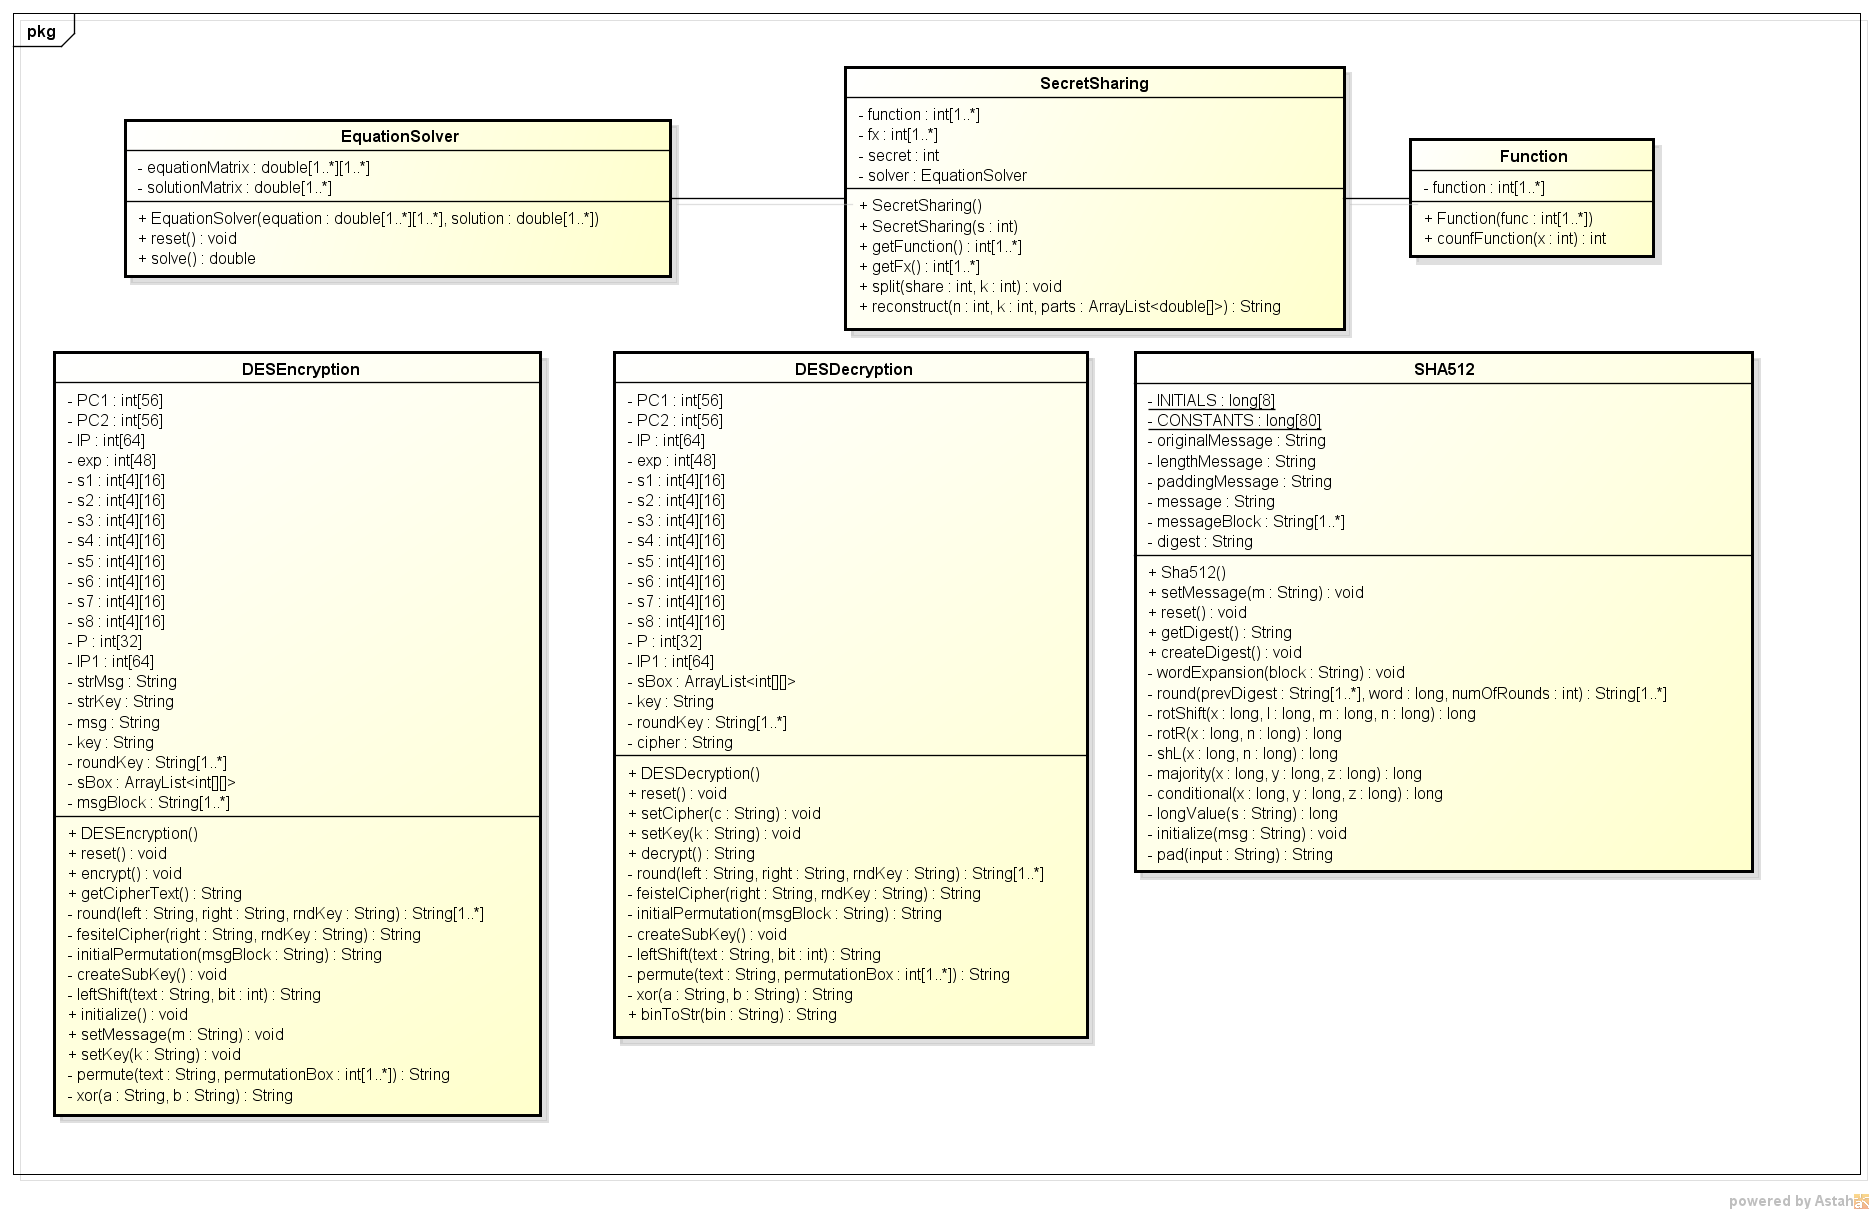
\includegraphics[scale=0.5]{Gambar/final_class_diagram}}
	%\caption{Diagram Kelas Rinci}\label{fig:final_class_diagram}
%\end{sidewaysfigure}

\begin{figure}[h]
	\centering
	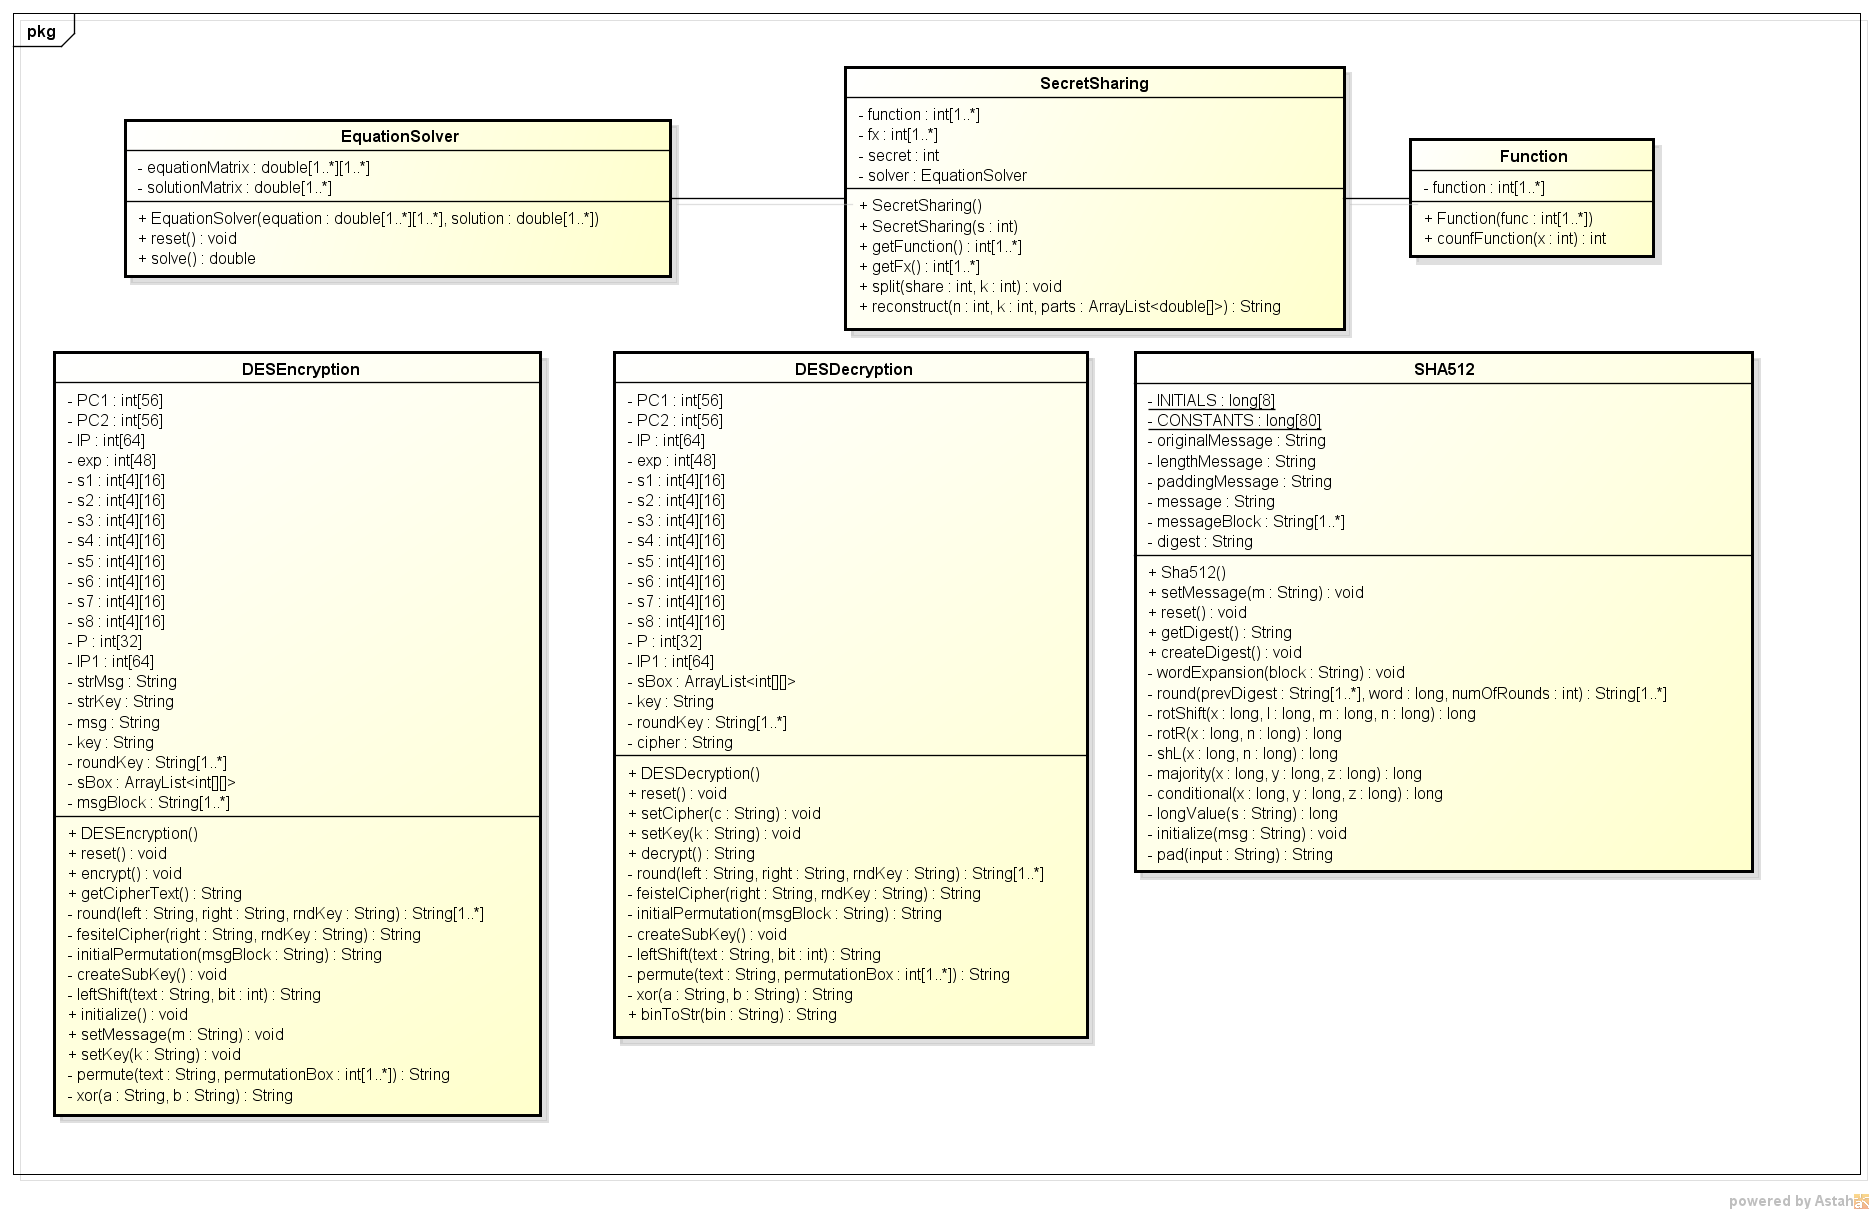
\includegraphics[angle=90, origin=c, scale=0.5]{Gambar/final_class_diagram}
	\caption{Diagram Kelas Rinci}\label{fig:final_class_diagram}
\end{figure}

\section{Deskripsi Kelas dan Fungsi}

Pada bagian ini akan berisi mengenai penjelasan secara rinci masing-masing kelas. Tujuannya adalah menjelaskan peran setiap kelas dalam perangkat lunak yang dibangun.

\subsection{Kelas \textit{SHA512}}

Kelas \textit{SHA512} merupakan kelas yang mengimplementasikan \textit{Secure Hashing Algorithm 512} (SHA-512). Cara kerja algoritma dapat dilihat pada bagian \ref{sec:SHA512}. Struktur kelas \textit{SHA512} ditunjukkan pada Gambar \ref{fig:classsha512}.

\begin{figure}[H]
	\centering
	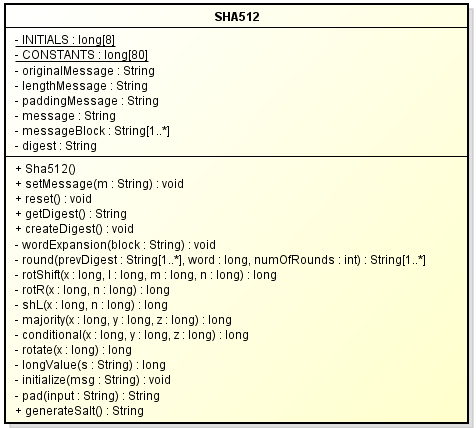
\includegraphics[scale=0.5]{Gambar/class_sha512}
	\caption{Kelas SHA512}\label{fig:classsha512}
\end{figure}

Adapun atribut dari kelas \textit{SHA512}, yaitu \textit{INITIALS, CONSTANTS, originalMessage, lengthMessage, paddingMessage, message, messageBlock,} dan \textit{digest}. Berikut penjelasan masing-masing atribut tersebut:

\begin{enumerate}
	\item \textit{long[8] INITIALS} \\
	Atribut yang berguna untuk menyimpan nilai dari konstanta awal.
	\item \textit{long[80] INITIALS} \\
	Atribut yang berguna untuk menyimpan konstanta yang digunakan dalam setiap putaran SHA-512.
	\item \textit{String originalMessage} \\
	Atribut yang berguna untuk menyimpan \textit{message} yang belum di\textit{padding} dalam bentuk \textit{string} biner.
	\item \textit{String lengthMessage} \\
	Atribut yang berguna untuk menyimpan informasi mengenai panjang atribut \textit{originalMessage} dalam bentuk \textit{string} biner.
	\item \textit{String paddingMessage} \\
	Atribut yang berguna untuk menyimpan blok \textit{padding} dalam bentuk \textit{string} biner.
	\item \textit{String message} \\
	Atribut yang berguna untuk menyimpan \textit{message} yang sudah di\textit{padding} dalam bentuk \textit{string} biner.
	\item String digest \\
	Atribut yang berguna untuk menyimpan \textit{digest} dari atribut \textit{message} dalam bentuk string \textit{biner}.
\end{enumerate}

Adapun fungsi yang membangun kelas \textit{SHA512}, yaitu \textit{Sha512, setMessage, reset, getDigest, wordExpansion, round, rotShift, rotR, shL, majority, conditional, rotate, longValue, initialize,} dan \textit{pad}. Berikut penjelasan masing-masing fungsi tersebut:

\begin{enumerate}
	\item \textit{Sha512} \\
	Merupakan konstruktor dari kelas \textit{SHA512}.
	\item \textit{void setMessage(String m)} \\
	Fungsi yang berguna untuk menyimpan nilai \textit{string m} ke dalam atribut \textit{originalMessage}.
	\item \textit{void reset} \\
	Fungsi yang berguna untuk mengembalikan nilai atribut \textit{originalMessage, lengthMessage, paddingMessage, message,} dan \textit{digest} menjadi \textit{string} kosong dan mengembalikan nilai atribut \textit{messageBlock} menjadi \textit{array string} kosong.
	\item \textit{String getDigest} \\
	Fungsi yang berguna untuk mengembalikan nilai atribut \textit{digest} dalam bentuk heksadesimal.
	\item \textit{void createDigest} \\
	Fungsi yang berperan untuk membuat \textit{digest} dari \textit{message}. Algoritma untuk membuat \textit{digest} ini dapat dilihat pada bagian \ref{sec:SHA512}.
	\item \textit{void wordExpansion(String block)} \\
	Fungsi yang berperan untuk melakukan proses ekspansi blok \textit{message}.
	\item \textit{String[] round(String[] prevDigest, long word, int numOfRounds)} \\
	Fungsi yang berperan untuk melakukan 1 putaran dari \textit{SHA512}. Proses yang terjadi dalam 1 putaran \textit{SHA512} dapat dilihat pada Bab \ref{sec:SHA512}.
	\item \textit{long rotShift(long x, long m, long n)} \\
	Fungsi yang berperan untuk melakukan operasi \begin{math}RotShift_{l-m-n}(x)\end{math} (Subbab \ref{subsec:expansiblokmsg}).
	\item \textit{long rotR(long x, long n)} \\
	Fungsi yang berperan untuk melakukan operasi \begin{math}RotR_i(x)\end{math} (Subbab \ref{subsec:expansiblokmsg}).
	\item \textit{long shL(long x, long n)} \\
	Fungsi yang berperan untuk melakukan operasi \begin{math}ShL_i(x)\end{math} (Subbab \ref{subsec:expansiblokmsg}).
	\item \textit{long majority(long x, long y, long z)} \\
	Fungsi yang berperan untuk melakukan operasi \begin{math}Majority(x,y,z)\end{math} (Subbab \ref{subsec:putaransha}).
	\item \textit{long conditional(long x, long y, long z)} \\
	Fungsi yang berperan untuk melakukan operasi \begin{math}Conditional(x,y,z)\end{math} (Subbab \ref{subsec:putaransha}).
	\item \textit{long rotate(long x)} \\
	Fungsi yang berperan untuk melakukan operasi \begin{math}Rotate(x)\end{math} (Subbab \ref{subsec:putaransha}).
	\item \textit{long longValue(String s)} \\
	Fungsi yang berperan mengubah tipe data \textit{string s} menjadi tipe data \textit{long}.
	\item \textit{void initialize(String msg)} \\
	Fungsi yang berperan untuk melakukan proses \textit{message padding} dan memecah menjadi blok-blok \textit{message}.
	\item \textit{String pad(String input)} \\
	Fungsi yang berperan untuk menambahkan \textit{padding} angka 0 pada \textit{string} biner \textit{input}. Algoritma fungsi ini ditunjukkan pada Algoritma \ref{padString}.
	
	\begin{algorithm}
		\caption{pad}
		\label{padString}
		\begin{algorithmic}[1]
			\Function{pad}{input}
				\If{\begin{math}input.length \: mod\: 8 != 0\end{math}}
					\State \begin{math}add = 8 - (input.length \: mod\: 8)\end{math}
				\EndIf
				\For{$i < add$}
					\State $res = res + "0"$
				\EndFor
				\State $res = res + input$
				\State \Return $res$
			\EndFunction
		\end{algorithmic}
	\end{algorithm}
	
\end{enumerate}

\subsection{Kelas \textit{Function}}

Kelas \textit{Function} merupakan kelas yang merepresentasikan sebuah fungsi polinomial \begin{math}f(x)\end{math}. Kelas \textit{Function} ditunjukkan pada Gambar \ref{fig:classfunction}.

\begin{figure}[H]
	\centering
	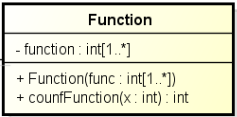
\includegraphics[scale=0.7]{Gambar/class_function}
	\caption{Kelas \textit{Function}}\label{fig:classfunction}
\end{figure}

Adapun atribut dari kelas \textit{Function} adalah \textit{function}. Atribut \textit{function} berguna untuk menyimpan nilai setiap koefesien dari fungsi polinomial \begin{math}f(x)\end{math} dalam tipe data \textit{array} bilangan bulat.

Sementara itu, fungsi yang dimiliki oleh kelas \textit{Function}, yaitu \textit{Function} dan \textit{countFunction}. Berikut penjelasan masing-masing fungsi:

\begin{enumerate}
	\item \textit{Function(int[] func)} \\
	Merupakan konstruktor dari kelas \textit{Function} yang menerima masukan \textit{array} bilangan bulat.
	\item \textit{int countFunction(int x)} \\
	Menghitung nilai \begin{math}x\end{math} untuk fungsi polinomial \begin{math}f(x)\end{math}. Algoritma dari fungsi ini ditunjukkan pada Algoritma \ref{countFunction}.
	\begin{algorithm}
		\caption{countFunction}
		\label{countFunction}
		\begin{algorithmic}[1]
			\Function{countFunction}{x}
				\For{$i < function.length$}
					\State \begin{math}res = res + (function[i]\: \cdot\: x^i)\end{math}
				\EndFor
				\State \Return \begin{math}res\end{math}
			\EndFunction
		\end{algorithmic}
	\end{algorithm}
\end{enumerate}

\subsection{Kelas \textit{EquationSolver}}

Kelas \textit{EquationSolver} adalah kelas yang mengimplementasikan eliminasi Gauss-Jordan (Bagian \ref{sec:eliminasigaussjordan}). Kelas ini berperan untuk menyelesaikan persamaan linear. Gambar \ref{fig:classequationsolver} menunjukkan struktur dari kelas \textit{EquationSolver}.

\begin{figure}[H]
	\centering
	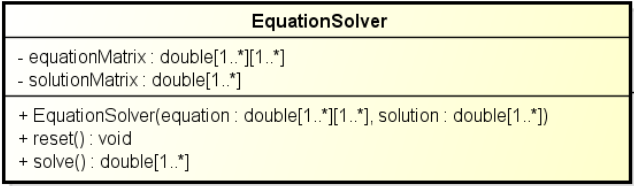
\includegraphics[scale=0.7]{Gambar/class_equation_solver}
	\caption{Kelas \textit{EquationSolver}}\label{fig:classequationsolver}
\end{figure}

Adapun atribut dari kelas \textit{EquationSolver}, yaitu \textit{equationMatrix} dan \textit{solutionMatrix}. Berikut penjelasan masing-masing atribut:

\begin{enumerate}
	\item \textit{double[][] equationMatrix} \\
	Atribut yang menyimpan bentuk matriks dari persamaan linear.
	\item \textit{double[] solutionMatrix} \\
	Atribut yang menyimpan bentuk matriks dari solusi masing-masing persamaan linear.
\end{enumerate}

Sementara itu, fungsi yang dimiliki oleh kelas \textit{EquationSolver}, yaitu \textit{EquationSolver}, \textit{reset}, dan \textit{solve}. Berikut penjelasan masing-masing fungsi:

\begin{enumerate}
	\item \textit{EquationSolver(double[][] equation, double[] solution)} \\
	Merupakan konstruktor dari kelas \textit{EquationSolver} yang menerima masukan berupa matriks persamaan dan matriks solusi.
	\item \textit{void reset} \\
	Mengembalikan nilai atribut \textit{equationMatrix} dan \textit{solutionMatrix} menjadi \textit{array} kosong.
	\item double[] solve \\
	Mencari solusi dari persamaan linear dan mengembalikan solusi dalam bentuk \textit{array}.
\end{enumerate}

\subsection{Kelas \textit{SecretSharing}}

Kelas \textit{SecretSharing} adalah kelas yang mengimplementasikan skema \textit{threshold(k,n)}. Kelas ini berperan untuk membangun \textit{share} dan juga merekonstruksi rahasia dari \textit{share}. Struktur kelas \textit{SecretSharing} ditunjukkan oleh Gambar \ref{fig:classsecretsharing}.

\begin{figure}[H]
	\centering
	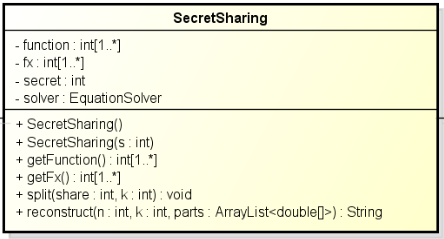
\includegraphics[scale=0.7]{Gambar/class_secret_sharing}
	\caption{Kelas \textit{DESEncryption}}\label{fig:classdesencryption}
\end{figure}

Kelas \textit{SecretSharing} memiliki beberapa atribut, yaitu \textit{function, fx, secret,} dan \textit{solver}. Berikut penjelasan masing-masing atribut:

\begin{enumerate}
	\item \textit{int[] function} \\
	Atribut yang menyimpan nilai setiap koefesien dari fungsi polinomial \begin{math}f(x)\end{math} dalam tipe data \textit{array} bilangan bulat.
	\item \textit{int[] fx} \\
	Atribut yang menyimpan nilai setiap koefesien dari rumus dasar fungsi \begin{math}f(x)\end{math} dalam tipe data \textit{array} bilangan bulat.
	\item \textit{int secret} \\
	Atribut yang menyimpan rahasia yang akan dibangun \textit{share-share}nya.
	\item \textit{EquationSolver solver} \\
	Atribut dari objek kelas \textit{EquationSolver}.
\end{enumerate}

Kelas \textit{SecretSharing} memiliki beberapa fungsi, yaitu \textit{SecretSharing, SecretSharing(int s), getFunction, getFx, split,} dan \textit{reconstruct}. Berikut penjelasan masing-masing fungsi:

\begin{enumerate}
	\item \textit{SecretSharing} \\
	Merupakan konstruktor kosong dari kelas \textit{SecretSharing}.
	\item \textit{SecretSharing(int s)} \\
	Merupakan konstruktor dengan masukan \textit{int s} yang akan disimpan ke dalam atribut \textit{secret}.
	\item \textit{int[] getFunction} \\
	Fungsi yang berguna untuk mengembalikan nilai atribut \textit{function}.
	\item \textit{int[] getFx} \\
	Fungsi yang berguna untuk mengembalikan nilai atribut \textit{fx}.
	\item \textit{split(int share, int k)} \\
	Fungsi yang berperan dalam proses pembangunan \textit{share-share}. Cara pembangunan \textit{share} dapat dilihat pada Bab \ref{sec:secretsharingshamir}.
	\item \textit{String reconstruct(int n, int k, ArrayList<double[]> parts)} \\
	Fungsi yang berperan dalam proses rekonstruksi rahasia dari \textit{share-share} yang dimiliki. \textit{Share-share} yang dimiliki ini disimpan dalam masukan \textit{ArrayList<double[]> parts}. Proses rekonstruksi rahasia dapat dilihat pada Bab \ref{sec:secretsharingshamir}.
\end{enumerate}

\subsection{Kelas \textit{DESEncryption}}

Kelas \textit{DESEncryption} adalah kelas yang mengimplementasikan algoritma \textit{Data Encryption Standard} (Bab \ref{sec:des}). Kelas ini berperan untuk melakukan proses enkripsi menggunakan \textit{Data Encryption Standard}. Struktur kelas \textit{DESEncryption} ditunjukkan oleh Gambar \ref{fig:classdesencryption}.

\begin{figure}[H]
	\centering
	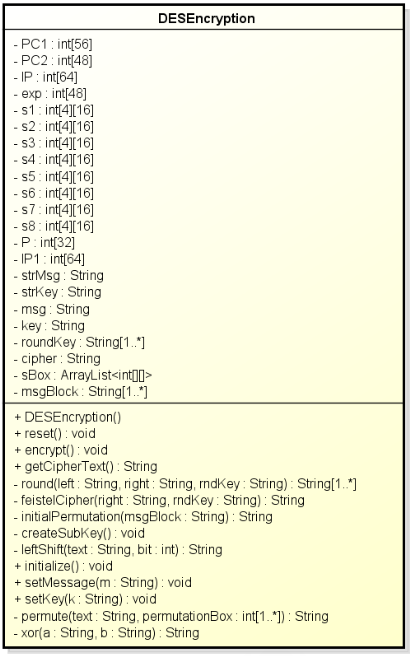
\includegraphics[scale=0.6]{Gambar/class_des_encryption}
	\caption{Kelas \textit{DESEncryption}}\label{fig:classdesencryption}
\end{figure}

Kelas DESEncryption memiliki beberapa atribut, yaitu \textit{PC1, PC2, IP, exp, s1, s2, s3, s4, s5, s6, s7, s8, P, IP1, strMsg, strKey, msg, key, roundKey, cipher, sBox,} dan \textit{msgBlock}. Berikut penjelasan masing-masing atribut:

\begin{enumerate}
	\item \textit{int[56] PC1} \\
	Atribut yang menyimpan matriks \textit{parity drop} yang digunakan dalam proses pembangkitan kunci putaran.
	\item \textit{int[48] PC2} \\
	Atribut yang menyimpan matriks permutasi \textit{P-box} yang digunakan dalam proses pembangkitan kunci putaran.
	\item \textit{int[64] IP} \\
	Atribut yang menyimpan matriks permutasi awal.
	\item \textit{int[48] exp} \\
	Atribut yang menyimpan matriks ekspansi \textit{P-box}.
	\item \textit{int[4][16] s1} \\
	Atribut yang menyimpan matriks \textit{s-box} ke-1.
	\item \textit{int[4][16] s2} \\
	Atribut yang menyimpan matriks \textit{s-box} ke-2.
	\item \textit{int[4][16] s3} \\
	Atribut yang menyimpan matriks \textit{s-box} ke-3.
	\item \textit{int[4][16] s4} \\
	Atribut yang menyimpan matriks \textit{s-box} ke-4.
	\item \textit{int[4][16] s5} \\
	Atribut yang menyimpan matriks \textit{s-box} ke-5.
	\item \textit{int[4][16] s6} \\
	Atribut yang menyimpan matriks \textit{s-box} ke-6.
	\item \textit{int[4][16] s7} \\
	Atribut yang menyimpan matriks \textit{s-box} ke-7.
	\item \textit{int[4][16] s8} \\
	Atribut yang menyimpan matriks \textit{s-box} ke-8.
	\item \textit{int[32] P} \\
	Atribut yang menyimpan matriks permutasi pada tahap terakhir fungsi DES.
	\item \textit{int[64] IP1} \\
	Atribut yang menyimpan matriks permutasi akhir.
	\item \textit{String strMsg} \\
	Atribut yang menyimpan \textit{plaintext} dalam bentuk \textit{string}.
	\item \textit{String strKey} \\
	Atribut yang menyimpan kunci dalam bentuk \textit{string}.
	\item \textit{String msg} \\
	Atribut yang menyimpan \textit{plaintext} dalam bentuk \textit{string} biner.
	\item \textit{String key} \\
	Atribut yang menyimpan kunci dalam bentuk \textit{string} biner.
	\item \textit{String[] roundKey} \\
	Atribut yang menyimpan kunci untuk setiap putaran dalam \textit{array string} biner.
	\item \textit{String cipher} \\
	Atribut yang menyimpan \textit{ciphertext} hasil enkripsi dalam bentuk \textit{string} biner.
	\item \textit{ArrayList<int[][]> sBox} \\
	Atribut yang menyimpan seluruh matriks \textit{s-box}.
	\item \textit{String[] msgBlock} \\
	Atribut yang menyimpan blok-blok \textit{plaintext} dalam bentuk \textit{array string} biner. Setiap elemen \textit{array} berisi \textit{string} biner dengan panjang 64-\textit{bit}.
\end{enumerate}

Adapun fungsi-fungsi yang dimiliki oleh kelas \textit{DESEncryption}, yaitu \textit{DESEncryption, reset, encrypt, getCipherText, round, feistelCipher, initialPermutation, createSubKey, leftShift, initialize, setMessage, setKey, permute,} dan \textit{xor}. Berikut penjelasan masing-masing fungsi:

\begin{enumerate}
	\item \textit{DESEncryption} \\
	Merupakan konstruktor dari kelas \textit{DESEncryption}.
	\item \textit{void reset} \\
	Fungsi yang berperan untuk mengembalikan atribut \textit{strMsg, strKey, msg, key,} dan \textit{cipher} menjadi \textit{string} kosong. Fungsi ini juga mengembalikan atribut \textit{roundKey} dan \textit{msgBlock} menjadi \textit{array string} kosong.
	\item \textit{void encrypt} \\
	Fungsi yang berperan untuk melakukan proses enkripsi DES.
	\item \textit{String getCipherText} \\
	Fungsi yang mengembalikan nilai atribut \textit{cipher} dalam bentuk \textit{string} heksadesimal.
	\item \textit{String[] round(String left, String right, String rndKey)} \\
	Fungsi yang berperan untuk melakukan 1 putaran dari DES. Fungsi ini mengembalikan \textit{array string} yang berguna untuk blok masukan putaran berikutnya.
	\item \textit{String feistelCipher(String right, String rndKey)} \\
	Fungsi yang berperan untuk melakukan proses jaringan Feistel kepada blok bagian kanan dari \textit{plaintext}.
	\item \textit{String initialPermutation(String msgBlock)} \\
	Fungsi ini berperan untuk melakukan proses permutasi awal.
	\item \textit{void createSubKey} \\
	Fungsi yang berperan untuk membangkitkan kunci putaran.
	\item \textit{String leftShift(String text, int bit)} \\
	Fungsi yang berperan untuk melakukan \textit{shift left} dari masukan \textit{string text} sebanyak masukan \textit{int bit}.
	\item \textit{void initialize} \\
	Fungsi yang berperan untuk melakukan \textit{padding} terhadap \textit{strMsg} dan memecah \textit{strMsg} menjadi blok-blok \textit{string}. Blok-blok \textit{string} ini akan disimpan pada atribut \textit{msgBlock}.
	\item \textit{void setMessage(String m)} \\
	Fungsi untuk menyimpan \textit{string m} ke dalam atribut \textit{strMsg}.
	\item \textit{void setKey(String k)} \\
	Fungsi untuk menyimpan \textit{string k} ke dalam atribut \textit{strKey}.
	\item \textit{String permute(String text, int[] permutationBox)} \\
	Fungsi yang berperan untuk melakukan proses permutasi.
	\item \textit{String xor(String a, String b)} \\
	Fungsi yang berperan untuk melakukan operasi XOR.
\end{enumerate}

\subsection{Kelas \textit{DESDecryption}}

Kelas \textit{DESDecryption} adalah kelas yang berperan untuk melakukan proses dekripsi menggunakan DES. Struktur kelas \textit{DESDecryption} ditunjukkan pada Gambar \ref{fig:classdesdecryption}.

\begin{figure}[H]
	\centering
	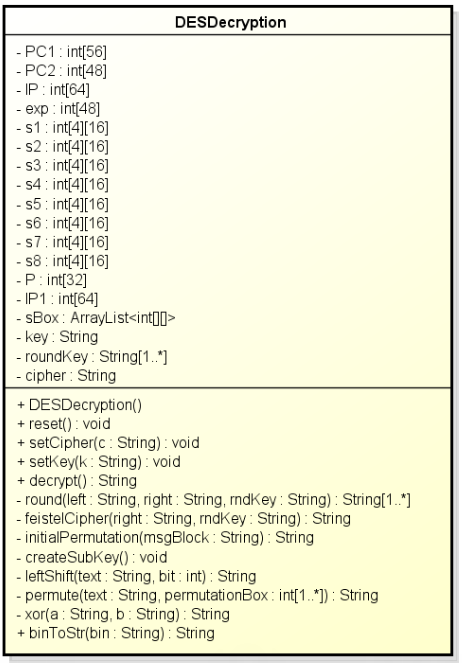
\includegraphics[scale=0.6]{Gambar/class_des_decryption}
	\caption{Kelas \textit{DESDecryption}}\label{fig:classdesdecryption}
\end{figure}

Kelas \textit{DESDecryption} memiliki beberapa atribut, yaitu \textit{PC1, PC2, IP, exp, s1, s2, s3, s4, s5, s6, s7, s8, P, IP1, sBox, key, roundKey,} dan \textit{cipher}. Berikut penjelasan masing-masing atribut:

\begin{enumerate}
	\item \textit{int[56] PC1} \\
	Atribut yang menyimpan matriks \textit{parity drop} yang digunakan dalam proses pembangkitan kunci putaran.
	\item \textit{int[48] PC2} \\
	Atribut yang menyimpan matriks permutasi \textit{P-box} yang digunakan dalam proses pembangkitan kunci putaran.
	\item \textit{int[64] IP} \\
	Atribut yang menyimpan matriks permutasi awal.
	\item \textit{int[48] exp} \\
	Atribut yang menyimpan matriks ekspansi \textit{P-box}.
	\item \textit{int[4][16] s1} \\
	Atribut yang menyimpan matriks \textit{s-box} ke-1.
	\item \textit{int[4][16] s2} \\
	Atribut yang menyimpan matriks \textit{s-box} ke-2.
	\item \textit{int[4][16] s3} \\
	Atribut yang menyimpan matriks \textit{s-box} ke-3.
	\item \textit{int[4][16] s4} \\
	Atribut yang menyimpan matriks \textit{s-box} ke-4.
	\item \textit{int[4][16] s5} \\
	Atribut yang menyimpan matriks \textit{s-box} ke-5.
	\item \textit{int[4][16] s6} \\
	Atribut yang menyimpan matriks \textit{s-box} ke-6.
	\item \textit{int[4][16] s7} \\
	Atribut yang menyimpan matriks \textit{s-box} ke-7.
	\item \textit{int[4][16] s8} \\
	Atribut yang menyimpan matriks \textit{s-box} ke-8.
	\item \textit{int[32] P} \\
	Atribut yang menyimpan matriks permutasi pada tahap terakhir fungsi DES.
	\item \textit{int[64] IP1} \\
	Atribut yang menyimpan matriks permutasi akhir.
	\item \textit{ArrayList<int[][]> sBox} \\
	Atribut yang menyimpan seluruh matriks \textit{s-box}.
	\item \textit{String key} \\
	Atribut yang menyimpan kunci dalam bentuk \textit{string} biner.
	\item \textit{String[] roundKey} \\
	Atribut yang menyimpan kunci untuk setiap putaran dalam \textit{array string} biner.
	\item \textit{String cipher} \\
	Atribut yang menyimpan \textit{ciphertext} yang akan didekripsi dalam bentuk \textit{string} biner.
\end{enumerate}

Adapun fungsi-fungsi yang dimiliki kelas \textit{DESDecryption}, yaitu \textit{DESDecryption, reset, setCipher, setKey, decrypt, round, feistelCipher, initialPermutation, createSubKey, leftShift, permute, xor,} dan \textit{binToStr}. Berikut penjelasan masing-masing fungsi:

\begin{enumerate}
	\item \textit{DESDecryption} \\
	Merupakan konstruktor dari kelas \textit{DESDecryption}.
	\item \textit{void reset} \\
	Fungsi yang berperan untuk mengembalikan atribut \textit{key} dan \textit{cipher} menjadi \textit{string} kosong. Fungsi ini juga mengembalikan atribut \textit{roundKey} menjadi \textit{array string} kosong.
	\item \textit{void setCipher(String c)} \\
	Fungsi untuk menyimpan \textit{string c} pada atribut \textit{cipher} dalam bentuk \textit{string} biner.
	\item \textit{void setKey(String k)} \\
	Fungsi untuk menyimpan \textit{string k} pada atribut \textit{key} dalam bentuk \textit{string} biner.
	\item \textit{String decrypt} \\
	Fungsi yang berperan untuk melakukan proses dekripsi menggunakan DES.
	\item \textit{String[] round(String left, String right, String rndKey)} \\
	Fungsi yang berperan untuk melakukan 1 putaran dari DES. Fungsi ini mengembalikan \textit{array string} yang berguna untuk blok masukan putaran berikutnya.
	\item \textit{String feistelCipher(String right, String rndKey)} \\
	Fungsi yang berperan untuk melakukan proses jaringan Feistel kepada blok bagian kanan dari \textit{plaintext}.
	\item \textit{String initialPermutation(String msgBlock)} \\
	Fungsi ini berperan untuk melakukan proses permutasi awal.
	\item \textit{void createSubKey} \\
	Fungsi yang berperan untuk membangkitkan kunci putaran.
	\item \textit{String leftShift(String text, int bit)} \\
	Fungsi yang berperan untuk melakukan \textit{shift left} dari masukan \textit{string text} sebanyak masukan \textit{int bit}.
	\item \textit{String permute(String text, int[] permutationBox)} \\
	Fungsi yang berperan untuk melakukan proses permutasi.
	\item \textit{String xor(String a, String b)} \\
	Fungsi yang berperan untuk melakukan operasi XOR.
	\item \textit{String binToStr(String bin)} \\
	Fungsi yang berperan untuk mengubah \textit{string} biner menjadi \textit{string}.
\end{enumerate}

\subsection{Kelas \textit{DataReader}}

Kelas \textit{DataReader} merupakan kelas yang berperan untuk membaca berkas teks. Kelas \textit{DataReader} ditunjukkan pada Gambar \ref{fig:classdatareader}.

\begin{figure}[H]
	\centering
	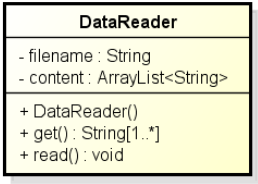
\includegraphics[scale=0.8]{Gambar/class_data_reader}
	\caption{Kelas \textit{DataReader}}\label{fig:classdatareader}
\end{figure}

Kelas ini memiliki 2 atribut, yaitu \textit{filename} dan \textit{content}. Berikut penjelasan masing-masing atribut:

\begin{enumerate}
	\item \textit{String filename} \\
	Atribut yang menyimpan nama dari berkas teks yang dibaca.
	\item \textit{ArrayList<String> content} \\
	Atribut yang menyimpan isi dari berkas teks yang dibaca.
\end{enumerate}

Adapun kelas ini memiliki 3 fungsi, yaitu \textit{DataReader, get,} dan \textit{read}. Berikut penjelasan masing-masing fungsi:

\begin{enumerate}
	\item \textit{DataReader} \\
	Merupakan konstruktor dari kelas \textit{DataReader}.
	\item \textit{String[] get} \\
	Fungsi yang berguna untuk mengembalikan atribut \textit{content}.
	\item \textit{void read} \\
	Fungsi yang berperan membaca berkas teks.
\end{enumerate}

\subsection{Kelas \textit{DataWriter}}

Kelas \textit{DataWriter} adalah kelas yang berperan untuk menulis keluaran ke dalam berkas teks. Kelas \textit{DataWriter} ditunjukkan pada Gambar \ref{fig:classdatawriter}.

\begin{figure}[H]
	\centering
	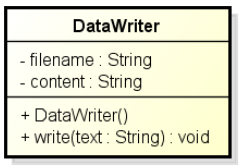
\includegraphics[scale=0.8]{Gambar/class_data_writer}
	\caption{Kelas \textit{DataWriter}}\label{fig:classdatawriter}
\end{figure}

Kelas ini memiliki 2 atribut, yaitu \textit{filename} dan \textit{content}. Berikut penjelasan masing-masing atribut:

\begin{enumerate}
	\item \textit{String filename} \\
	Atribut yang menyimpan nama dari berkas teks yang akan ditulis.
	\item \textit{String content} \\
	Atribut yang menyimpan isi dari berkas teks yang akan ditulis.
\end{enumerate}

Adapun kelas ini memiliki 2 fungsi, yaitu DataWriter dan write. Berikut penjelasan masing-masing fungsi:

\begin{enumerate}
	\item DataWriter \\
	Merupakan konstruktor dari kelas \textit{DataWriter}.
	\item \textit{write(String text)} \\
	Fungsi yang berperan untuk menulis isi dari berkas teks.
\end{enumerate}

\section{Perancangan Antarmuka}

Perangkat lunak yang dikembangkan akan memiliki 3 tampilan utama, tampilan untuk menyimpan \textit{password}, tampilan untuk mengembalikan \textit{password}, dan tampilan untuk memilih menyimpan \textit{password} atau mengembalikan \textit{password}.

Gambar \ref{fig:tampilan-awal} menunjukkan tampilan awal yang akan dimunculkan pertama kali untuk memilih menyimpan \textit{password} atau mengembalikan \textit{password}.

%diagram
\begin{figure}[H]
	\centerline{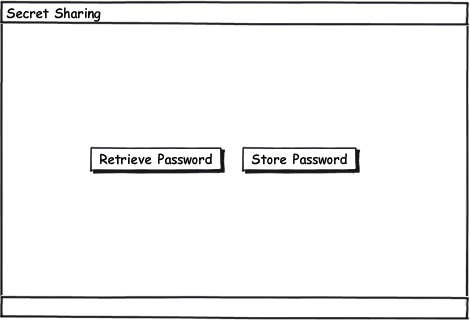
\includegraphics[scale=0.5]{Gambar/tampilan-utama}}
	\caption{Perancangan Tampilan Awal}\label{fig:tampilan-awal}
\end{figure}

Tampilan utama ini cukup sederhana. Dalam tampilan utama pada Gambar \ref{fig:tampilan-awal}, hanya terdapat 2 pilihan, yaitu \textit{store password} untuk menyimpan \textit{password} dan \textit{retrieve password} untuk mengembalikan \textit{password}. Selanjutnya, jika pengguna memilih \textit{store password}, maka akan ditampilkan halaman \textit{store password}.

%diagram
\begin{figure}[H]
	\centerline{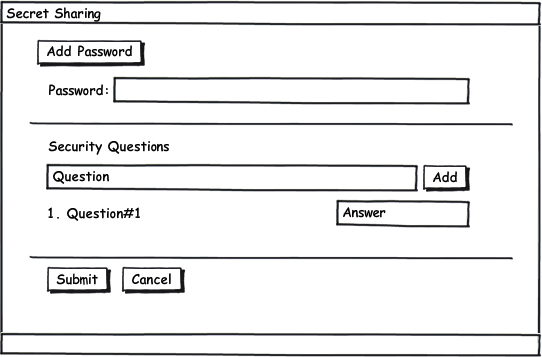
\includegraphics[scale=0.5]{Gambar/store_password}}
	\caption{Perancangan Tampilan Menyimpan \textit{Password}}\label{fig:store_password}
\end{figure}

Pada tampilan menyimpan \textit{password} di Gambar \ref{fig:store_password}, tombol "\textit{Add Password}" berfungsi untuk menambah \textit{text box password}, pada bagian ini pengguna bisa mengisi \textit{password} yang akan disimpan. Bagian "\textit{Security Questions}" berisi pertanyaan keamanan yang dibuat oleh pengguna. Setelah pengguna mengisi pertanyaan personal pada \textit{text box} di bagian "\textit{Security Questions}" dan menekan tombol "\textit{Add}", akan muncul pertanyaan yang sudah dibuat, kemudian pengguna harus mengisi jawaban dari pertanyaan keamanan yang sudah dibuat.

Setelah mengisi seluruh pertanyaan keamanan, pengguna bisa menyimpan \textit{password} dengan menekan tombol "\textit{Submit}". Tombol "\textit{Cancel}" berfungsi untuk kembali ke tampilan awal. Setelah tombol "\textit{Submit}" ditekan, maka \textit{password} sudah disimpan dan akan kembali ditampilkan tampilan awal.

Berikutnya adalah tampilan untuk mengembalikan \textit{password}. Gambar \ref{fig:retrieve_password} menunjukkan tampilan untuk mengembalikan \textit{password}.

%diagram
\begin{figure}[H]
	\centerline{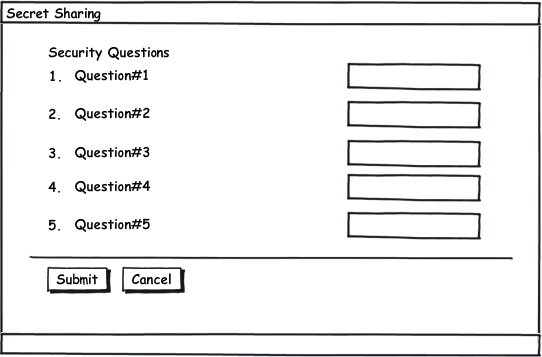
\includegraphics[scale=0.5]{Gambar/retrieve_password}}
	\caption{Perancangan Tampilan Mengembalikan \textit{Password}}\label{fig:retrieve_password}
\end{figure}

Pada bagian untuk mengembalikan \textit{password}, tampilannya cukup sederhana dan pengguna hanya cukup memasukkan setiap jawaban dari pertanyaan keamanan yang sudah dibuat sebelumnya di bagian penyimpanan password. Pada bagian ini, pengguna bebas untuk memilih mengisi setiap pertanyaan atau tidak menjawab pertanyaan keamanan. Setelah seluruh pertanyaan sudah dijawab, pengguna dapat menekan tombol "\textit{Submit}" yang kemudian akan menunjukkan \textit{password} pengguna.

Gambar \ref{fig:password} menunjukkan tampilan sesudah pengguna menekan tombol "\textit{Submit}" pada bagian di Gambar \ref{fig:retrieve_password}.

%diagram
\begin{figure}[H]
	\centerline{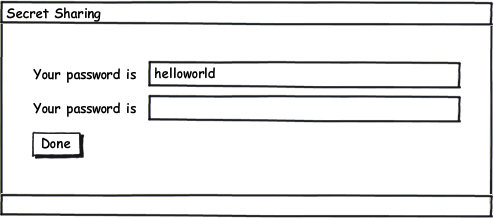
\includegraphics[scale=0.5]{Gambar/password}}
	\caption{Perancangan Tampilan Mengembalikan \textit{Password} (2)}\label{fig:password}
\end{figure}

Jika banyak pertanyaan keamanan yang dijawab benar oleh pengguna sesuai dengan minimal banyak pertanyaan keamanan yang dijawab benar maka pengguna bisa melihat \textit{password} yang sudah disimpan. Tapi, jika banyak pertanyaan keamanan yang dijawab benar oleh pengguna kurang dari minimal banyak pertanyaan keamanan yang harus dijawab benar maka pengguna tidak bisa melihat \textit{password} yang sudah disimpan.